\documentclass[journal]{vgtc}                % final (journal style)
%\documentclass[review,journal]{vgtc}         % review (journal style)
%\documentclass[widereview]{vgtc}             % wide-spaced review
%\documentclass[preprint,journal]{vgtc}       % preprint (journal style)

%% Uncomment one of the lines above depending on where your paper is
%% in the conference process. ``review'' and ``widereview'' are for review
%% submission, ``preprint'' is for pre-publication, and the final version
%% doesn't use a specific qualifier.

%% These few lines make a distinction between latex and pdflatex calls and they
%% bring in essential packages for graphics and font handling.
%% Note that due to the \DeclareGraphicsExtensions{} call it is no longer necessary
%% to provide the the path and extension of a graphics file:
%% 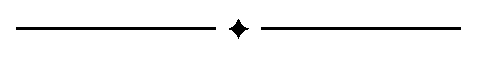
\includegraphics{diamondrule} is completely sufficient.
%%
\ifpdf%                                % if we use pdflatex
  \pdfoutput=1\relax                   % create PDFs from pdfLaTeX
  \pdfcompresslevel=9                  % PDF Compression
  \pdfoptionpdfminorversion=7          % create PDF 1.7
  \ExecuteOptions{pdftex}
  \usepackage{graphicx}                % allow us to embed graphics files
  \DeclareGraphicsExtensions{.pdf,.png,.jpg,.jpeg} % for pdflatex we expect .pdf, .png, or .jpg files
\else%                                 % else we use pure latex
  \ExecuteOptions{dvips}
  \usepackage{graphicx}                % allow us to embed graphics files
  \DeclareGraphicsExtensions{.eps}     % for pure latex we expect eps files
\fi%

%% it is recomended to use ``\autoref{sec:bla}'' instead of ``Fig.~\ref{sec:bla}''
\graphicspath{{figures/}{pictures/}{images/}{./}} % where to search for the images
\usepackage{xcolor}

\usepackage{microtype}                 % use micro-typography (slightly more compact, better to read)
\PassOptionsToPackage{warn}{textcomp}  % to address font issues with \textrightarrow
\usepackage{textcomp}                  % use better special symbols
\usepackage{mathptmx}                  % use matching math font
\usepackage{times}                     % we use Times as the main font
\renewcommand*\ttdefault{txtt}         % a nicer typewriter font
\usepackage[sort]{cite}

%% If you are submitting a paper to a conference for review with a double
%% blind reviewing process, please replace the value ``0'' below with your
%% OnlineID. Otherwise, you may safely leave it at ``0''.
\onlineid{0}

%% declare the category of your paper, only shown in review mode
\vgtccategory{Research}

%% Paper title - 1 pt for descriptive title
\title{Interactive visualization techniques to represent Covid correlation data using choropleth}

%% This is how authors are specified in the journal style

%% indicate IEEE Member or Student Member in form indicated below
%% 1 pt for name
\author{Ashwini Kurady}
\authorfooter{
%% insert punctuation at end of each item
\item
 Ashwini Kurady is a graduate student at the University of Arizona. E-mail:ashwinikurady@email.arizona.edu.
}

%other entries to be set up for journal
%\shortauthortitle{Firstauthor \MakeLowercase{\textit{et al.}}: Paper Title}

%% Abstract section - 5 pts
\abstract{
The spread of Covid-19 has brought the world to a standstill. In these times, creating awareness about the pandemic is of tantamount importance. Data visualization, in particular, has the ability to present the complex data comprising numbers in human-readable simple format. This project aims towards interactive visualization and choropleth mapping of Northern America in showing the impact of COVID data and even helps to derive dependencies on different factors like mode of spreading, correlation between different metrics of data and also the dependence on demographics.
} % end of abstract

%% Keywords that describe your work. Will show as 'Index Terms' in journal
%% please capitalize first letter and insert punctuation after last keyword
%\keywords{Radiosity, global illumination, constant time}

%% ACM Computing Classification System (CCS). 
%% See <http://www.acm.org/class/1998/> for details.
%% The ``\CCScat'' command takes four arguments.

%\CCScatlist{ % not used in journal version
% \CCScat{K.6.1}{Management of Computing and Information Systems}%
%{Project and People Management}{Life Cycle};
% \CCScat{K.7.m}{The Computing Profession}{Miscellaneous}{Ethics}
%}

%% Uncomment below to include a teaser figure.
%   \teaser{
%   \centering
%   \includegraphics[width=16cm]{CypressView}
%   \caption{In the Clouds: Vancouver from Cypress Mountain.}
%  }

%% Uncomment below to disable the manuscript note
%\renewcommand{\manuscriptnotetxt}{}

%% Copyright space is enabled by default as required by guidelines.
%% It is disabled by the 'review' option or via the following command:
% \nocopyrightspace

\vgtcinsertpkg

%%%%%%%%%%%%%%%%%%%%%%%%%%%%%%%%%%%%%%%%%%%%%%%%%%%%%%%%%%%%%%%%
%%%%%%%%%%%%%%%%%%%%%% START OF THE PAPER %%%%%%%%%%%%%%%%%%%%%%
%%%%%%%%%%%%%%%%%%%%%%%%%%%%%%%%%%%%%%%%%%%%%%%%%%%%%%%%%%%%%%%%%

\begin{document}

%% The ``\maketitle'' command must be the first command after the
%% ``\begin{document}'' command. It prepares and prints the title block.

%% the only exception to this rule is the \firstsection command
\firstsection{Introduction} % or "Motivation"

\maketitle

COVID-19 has taken the world by storm in the year 2020. It has wreaked havoc in lives of everyone on the planet and re-defined human interaction. It also has caused the death of more than a million people across the planet. It is in these trying times that the impact of technology \& the responsibility on it increase multi-fold. In particular, data visualization has a large role to play due to its ability to present the results of scientific analysis to the general public. A good visualization can present trends in data which might not be visible from numbers and help the layman appreciate the urgency of the situation better. It can help ensure that each additional life lost due to COVID is not just another number added to the total, but actually serves the purpose of increasing the awareness in others.

There is already a plethora of websites online detailing numbers related to COVID-19 and quite a few of those have very interactive data visualizations to help better analyze the data. A majority of them focus on presenting the data in pie/bar chart form which provides for good viewing of data. However, this does not help to solve the inherent issue with data bias. For ex, just looking at the raw data in terms of COVID cases does not do justice to the impact of population density, per capita income and other demographics on the spread. It is important to take all the factors into account while presenting the visualization of the case spread. This would aid in creating better awareness about the ease of COVID spread.

Due to the interdependence of data, it is important to look at the correlation to all metrics. A correlation plot like a small multiple plot can help to present this interdependence of data better. Adding interaction helps the user to choose and view the data of his/her choice. Another very useful approach is to have a cartographic map of this correlated data to help people analyze the data for the regions of their interest. Some might think that Cartography is showing the map using different colors and make them look visually stunning but Cartography is both science and art form of study of maps. Choropleth maps help to better visualize the data by showing the relative scores for different regions of interest.

With the rise of COVID cases in the USA due to the third wave, there is an increased emphasis on the need for better visualization tools to create further awareness among the general public. The project concentrates on how to apply the dataset of COVID cases on the map of USA based on both the raw data and per capita cases using its spatial information and its layout. As we are integrating the non-spatial data such as number of people recovered, regions or states mostly affected, people who have died from the virus and many other contexts with base spatial data i.e., map of the USA, this project will be based on choropleth mapping techniques.

The objectives of this project are:
\begin{itemize}
  \item to perform a comprehensive analysis of the existing data visualization techniques for COVID-19
  \item to develop a choropleth map based visualization tool to better visualize COVID-19 spread and its correlation to different parameters like per capita
  \item to provide a better tool to the general public and help to create more awareness via these visualizations
\end{itemize}
 

%Background and Related Work: 20%

\section{Background}
\label{sec:background}


Below mentioned are few of the works which were helpful in understanding the usage of choropleth. An example of the command-line cartography using choropleth for population density is shown in \cite {med}. Another example of the visualization of the United States election results which have an accepted standard representation of red and blue pattern in cartography is demonstrated in \cite{NYT}. An example of Zoom in feature for choropleth which helps in differentiating the visualization pattern for states and counties is shown in \cite{cmgiven}. Despite the popularity of the cartography and its variants, it is important to explore the tasks suitable for the cartography based on visualization goals. This project will be implemented using the cartography map in choropleth. The project will describe the covid cases based on per capita of each state on cartography. Terminologies In this project include: 1. Per capita category: covid cases in each state with relation to the category choose for the state. Choosing choropleth helps to better demonstrate the visualization and helps to better interpret the data. The main goal of the project is to showcase the correlation data for covid19 cases such as those based on per capita. Many of the covid19 visualization give details on cases in each county but does not compare the severity using per capita. This project focus on building the relationship between the population in each state and number of categories in covid cases in the state which will truly show the severity.

\subsection{Related Work}
\label{sec:related}


\cite{choroUn} shows an example of implementation of choropleth maps for unemployment data for different states in the United States. However, the way it is implemented, the algorithm is hard-coded for the data format and can only handle one datapoint. 

Interactive web visualization is presented in \cite{covidviz} employing a knee detection algorithm to categorize based on duration of COVID spread. While this presents a very effective data visualization and segregation, the data considered is raw data without considering per capita data and hence is subjective. Critical trends showing the live tracking of global covid cases and fatalities as shown in \cite{jhu}. This shows very detailed data split up based on states within individual countries as shown in Figure \ref{fig:JHU_Covid}. However, the drawback of this approach is the absence of any correlation data between different parameters. The user has to derive the correlation separately looking at the different plots and cartographic maps.

\begin{figure}[h]
 \centering % avoid the use of \begin{center}...\end{center} and use \centering instead (more compact)
 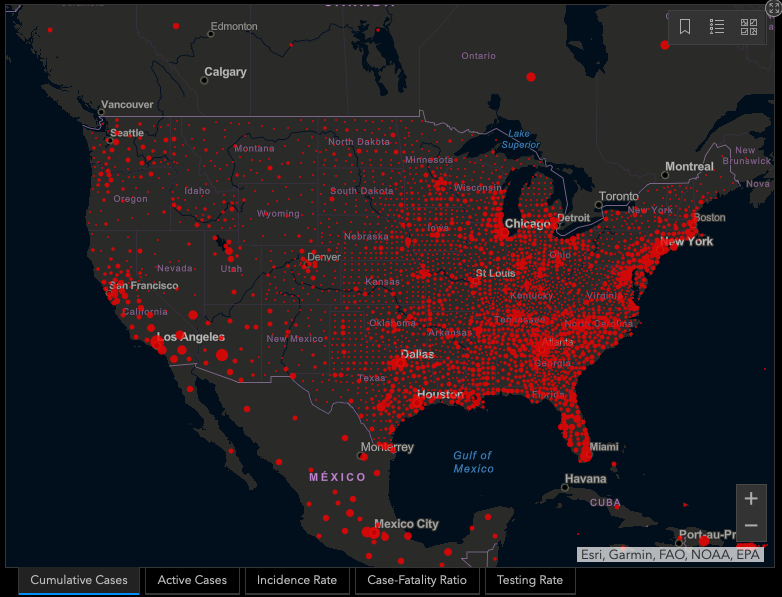
\includegraphics[width=3in]{figs/JHU_Covid.png}
 \caption{Cartographic map of Covid spread}
 \label{fig:JHU_Covid}
\end{figure}


%Research Plan - 20%
\section{Research Plan} 
\label{sec:research}

Given the ever-growing flood of information, Cartography provide an visually appealing way to present the world reality. The approach of this project is to visualize covid cases among different states of Northern America on the basis of per capita using cartographic mapping. 
The visualization of the covid pandemic can be classified as two types, static visualization \cite{WaPo} and complex interactive visualization \cite{CovViz} which gives overall perspective but hinder to provide details required for the user  to go in deep for the particular region and how the region is affected. This project aims to include interactive visualization and provide details of each region in the northern America on the basis of proportional statistics ie; there will be clear distinction between the severity or improvement in cases based on universal scaling and on the other hand calculating the number of cases based on total number of people in the region. 
According to work presented by Zhou et al. \cite{Zhou}, they categorize “visualization technique” as low level operation and “visual task” as interface between the visual representation and visual techniques without specifying “how” an operation is done. This project aims to facilitate both these categorization by implementing cartography based on two components such as population of each state and different metrics of covid cases in each state. In order to show the metrics such as positive cases, negative cases, total tests, recovery cases and number of death from covid in each state, we have included the mouse hover effect interaction through which, by hovering over the states, we can show details of all the metrics of the respective state. Sequential color scheme has been implemented to forecast the impact of covid and changes as per naïve data and per capita data for each metric. This project is implemented using interactive visualization for mouseover, click, mouseout and button based interactions.

\begin{figure}[h]
 \centering % avoid the use of \begin{center}...\end{center} and use \centering instead (more compact)
 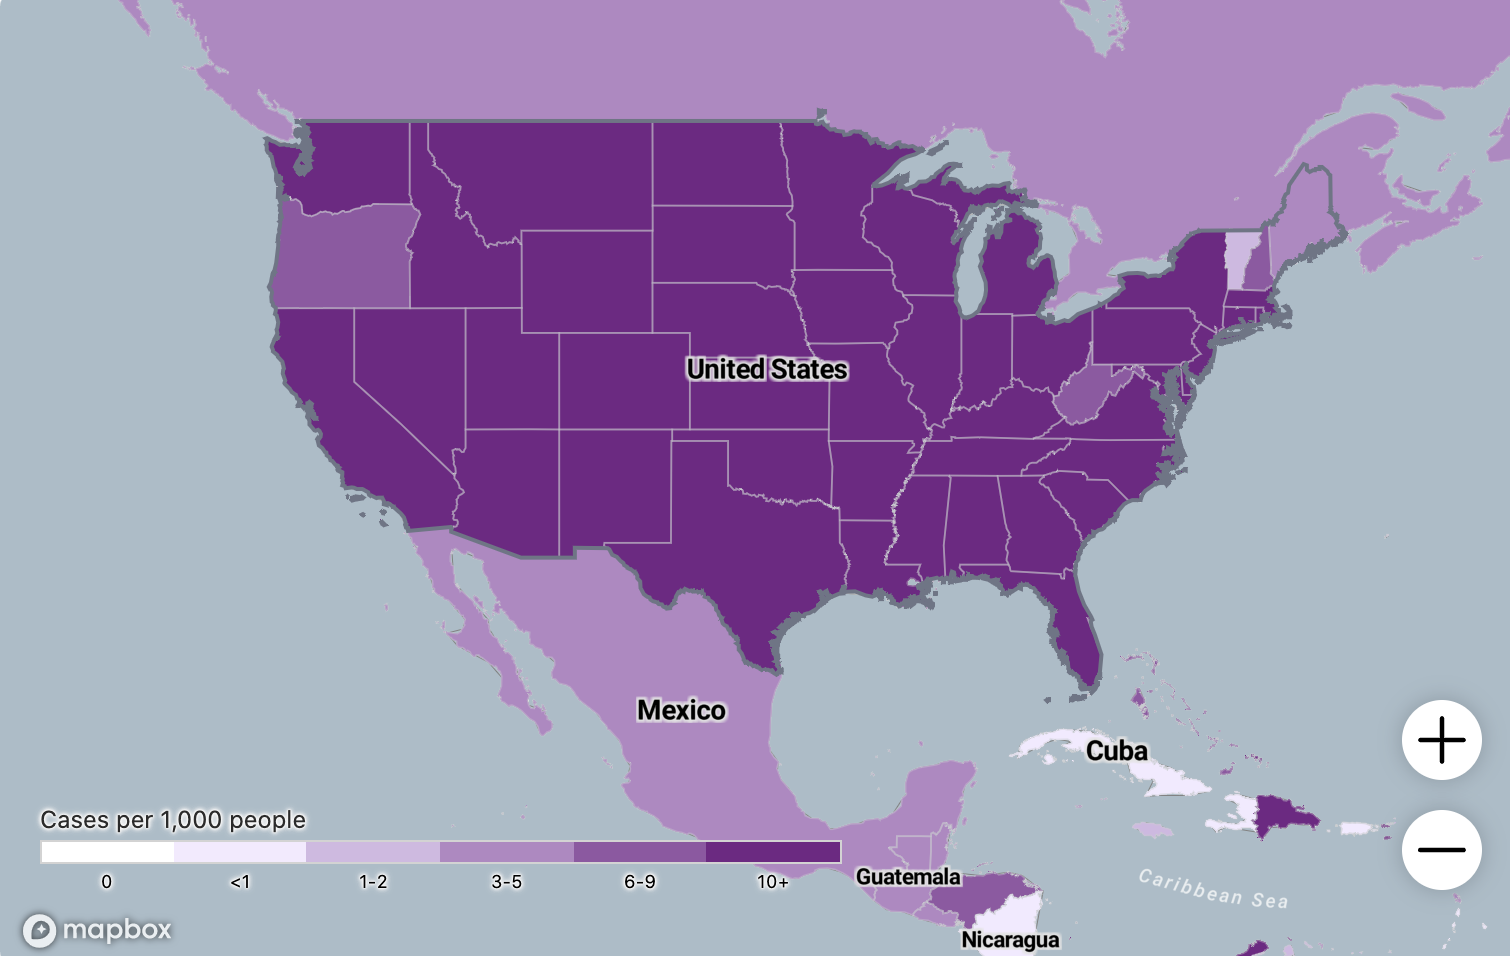
\includegraphics[width=3in]{figs/Weatherdata.png}
 \caption{Choropleth map for weather data \cite{Weather}}
 \label{fig:weather}
\end{figure}

\subsection{Data}
\label{sec:data}

Data for this project is taken from the COVID Tracking Project \cite{CTP}. This dataset includes the latest Covid-19 statistics from March till date and is updated daily. The data is categorized state-wise and shows different parameters including number of positive cases, number of negative cases etc. Population data of USA has been taken from a reference lookup table \cite{PopData}. This dataset includes total population of the country and categorized from highest to lowest as per state according to the population. 

\subsection{Evaluation}
\label{sec:eval}

The project can be evaluated on the basis of the milestones as shown in the timeline section. Some metrics for evaluation can be – efficacy of the cartographic mapping technique in showing the covid spread, the correlation plots between different categories and the implementation of additional features like mousein, mouseout, zoom etc.
Another metric is to evaluate the flexibility of the implemented visualization technique to handle changes in data since the data can change quite quickly. The visualization technique has to ensure that overcrowding doesn’t happen due to the saturation of datapoints and this becomes a key metric to ensure the data is well presented.

\subsection{Technology}
\label{sec:tech}

As D3 \cite{d3js} supports web mapping and interaction and also supports topology projection. This project will be implemented using d3.js and HTML5 and Using Topojson library \cite{top} to encode the topology. 
Above mentioned list of technologies are extremely powerful when it comes for handling geographical information. 





% Impact - 20%
\section{Impacts}
\label{sec:impact}

Though there are a ton of COVID related visualization tools \& websites, but the aim of this project is to create a visualization tool that will help users to derive correlation data between different metrics using cumulative plots for easy comparison and present the complex data in a simplified manner by helping with an option to check the covid spread based on per-capita to the general public.  
\subsection{Conclusion}
\begin{itemize}
\item Anyone using this tool should be able to get a feel for the general state of covid spread in the region that they are in through choropleth mapping techniques. 
\item The implementation of interactive visualization implemented in this project aids in better understanding the correlation between different factors impacting the spread of Covid. 
\item By providing an option to showcase per-capita data for each state and as well as compare between with and without percapita scenarios, this project helps to show the actual severity/recovered scenario of the states which is rare to find in other similar implementation.
\item Multi-data handling can be added to also show county data along with state wise data. However, this will have to take care of inherent data bias since the data sources for the two are different and ensuring proper weights to each data will be crucial.
\end{itemize}

\subsection{Future improvement}
One avenue to improve the visualization tool presented here is in handling the data. While this tool can handle data on the fly, more exception handling can be added to handle cases where numbers might not have been reported by individual states. Addition of slider based animation tools to show cumulative information on choropleth map is another possible improvement.



%\bibliographystyle{abbrv}
\bibliographystyle{abbrv-doi-hyperref}
%%use following if all content of bibtex file should be shown
%\nocite{*}
\bibliography{final}
\end{document}

